\section{March 05:}

\subsection{Length function}

    Let \(A\) be a ring, and \(M\) a f.g. \(A\)-module. 
    By the Jordan-Hölder theorem, if \(M\) has a filtration 
    \[
        M = M_0 \supset M_1 \supset \cdots \supset M_r = 0
    \]
    such that each \(M_i/M_{i+1} \cong A/\frakm_i\) for some maximal ideal \(\frakm_i\), 
    then the length \(r\) does not depend on the choice of the filtration.
    We call the \(r\) the \emph{length} of \(M\), denoted by \(\call_A(M)\).
    Otherwise, we say \(\call_A(M) = \infty\).

    If \(A\) an Artinian ring, then any f.g. \(A\)-module has finite length.

    \begin{example}
        Let \(A\) be a DVR, \(r \neq 0 \in A\).
        Then \(A/(r) \cong A/\frakm^{\nu(r)}\), where \(\nu\) is the valuation of \(A\).
        Then we have a filtration
        \[
            A/(r) = A/\frakm^{\nu(r)} \supset A/\frakm^{\nu(r)-1} \supset \cdots \supset A/\frakm \supset 0
        \]
        of length \(\nu(r)\) with successive quotients isomorphic to \(A/\frakm\).
        So \(\call_A(A/(r)) = \nu(r)\).
    \end{example}

    \begin{lemma}[{See \cite[A.3.1]{Fulton13Intersection}}]\label{lem:length_of_extension}
        Let \(A\) be a \(1\)-dimensional local noetherian domain with \(\KK = \Frac(A)\).
        Let \(B\) be the integral closure of \(A\) in \(\KK\).
        Then \(B\) is a Dedekind domain.
        Assume \(B\) is a f.g. \(A\)-module, then \(\forall r \neq 0 \in A\), we have 
        \[ \call_A(A/rA) = \sum_{\frakm \in \mSpec B} \call_{B_\frakm}(B_\frakm/rB_\frakm)[B/\frakm : A/\frakm_A]. \]
    \end{lemma}

    Apply Lemma \ref{lem:length_of_extension} to \(A = \calO_{X,V}\), where \(X\) is a variety and \(V\) is a subvariety of codimension \(1\).
    Then for all \(r = a/b \in \fkk(X)^\times\) with \(a,b \in \calO_{X,V}\), we have
    \[ \ord_V(r) = \call_{\calO_{X,V}}(\calO_{X,V}/(a)) - \call_{\calO_{X,V}}(\calO_{X,V}/(b)). \]

    \begin{example}
        Let \(X = \{y^2 = x^3\} \subset \bbA^2\) be a cuspidal cubic curve, and \(O = \{(0,0)\}\) be the cusp.
        Then \(\fkk(X) = \Frac \kk[x,y]/(y^2-x^3) \cong \Frac \kk[t]\) via \(x \mapsto t^2, y \mapsto t^3\).
        Compute:
        \[ \ord_O(x) = \call_{\calO_{X,O}}(\calO_{X,O}/(x)) = \call_{\calO_{X,O}}(\kk[x,y]/(x,y^2-x^3)) = \dim_\kk \kk[x,y]/(x,y^2) = 2. \]
        Hence 
        \[ \divisor(x) = 2[O]. \]
        Similarly, we have 
        \[ \divisor(y) = 3[O]. \]
    \end{example}

    \begin{definition}
        Let \(X\) be a scheme, \(X_1, \ldots, X_t\) be the irreducible components of \(X\).
        Define the \emph{fundamental cycle} of \(X\) to be
        \[ [X] = \sum_{j=1}^t \call(\calO_{X,X_j}) [X_j]. \]
        The length \(\call(\calO_{X,X_j})\) is called the \emph{generic multiplicity} of \(X_j\) in \(X\).
    \end{definition}

    \begin{example}
        Let \(X = \{x^3y^2(x^2+y^2-1) = 0\} \subset \bbA^2\).
        Then \(X\) has three irreducible components \(X_1 = \{x=0\}, X_2 = \{y=0\}, X_3 = \{x^2+y^2-1=0\}\).
        \begin{center}
            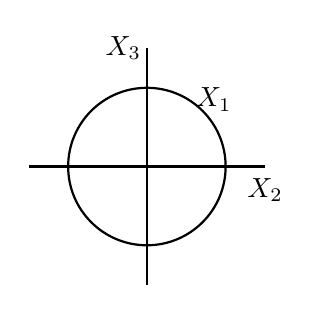
\begin{tikzpicture}[scale=1]
                % Circle
                \draw[thick] (0,0) circle (1);
                % x-axis
                \draw[thick] (-1.5,0) -- (1.5,0);
                % y-axis
                \draw[thick] (0,-1.5) -- (0,1.5);
                % Labels: X_1 for circle, X_2 for x-axis (y=0), X_3 for y-axis (x=0)
                \node at (0.85,0.85) {$X_1$};
                \node at (1.5,-0.3) {$X_2$};
                \node at (-0.3,1.5) {$X_3$};
            \end{tikzpicture}
        \end{center}
        We have:
        \[ \call(\calO_{X,X_1}) = \call\left(\left(\kk[x,y]/(x^3y^2(x^2+y^2-1))\right)_{(x)}\right) = \dim_{\kk(y)} \kk(y)[x]/(x^3) = 3. \]
        Similarly, we have \(\call(\calO_{X,X_2}) = 2\) and \(\call(\calO_{X,X_3}) = 1\).
        Hence
        \[ [X] = 3[X_1] + 2[X_2] + [X_3]. \]
    \end{example}

    \begin{proposition}\label{prop1}
        Let \(X\) be a scheme, \(\alpha \in Z_i(X)\).
        Then \(\alpha \sim 0\) if and only if there exist finitely many subvarieties of dimension \(i+1\) of \(\bbP^1 \times X\), say \(W_1, \ldots, W_r\), 
        such that the projection \(W_j \to \bbP^1\) is dominant for all \(j\), and
        \[ \alpha = \sum_{j=1}^r [f_j^{-1}(0)] - [f_j^{-1}(\infty)]. \]
    \end{proposition}
    \begin{proof}[Ideal of Proof]
        For a variety \(V\) and a dominant morphism \(f : V \to \bbP^1\), the divisor of \(f\) is just \(\divisor(f) = [f^{-1}(0)] - [f^{-1}(\infty)]\).

        For a subvariety \(V' \subset X\) and \(f' \in \fkk(V')^\times\), apply the above result to the closure of the graph \(\Gamma\) of \(f'\) in \(V' \times \bbP^1\).
        Note that \(\Gamma \to V'\) is birational.
        % \Yang{}
    \end{proof}

    \begin{example}
        As an application of \cref{prop1}, one can show 
        \[ \CH_i(\bbA^n) = \begin{cases}
            \bbZ\cdot[\bbA^n], & i = n, \\
            0, & i < n.
        \end{cases} \]
        (left as an exercise)
    \end{example}

\subsection{Flat pullbacks}
    
    Let \(f : X \to Y\) be a flat morphism of schemes of relative dimension \(n\).
    In this class, by a \emph{flat morphism}, we always mean a flat morphism of constants relative dimension.
    Here are examples that we should keep in mind:
    \begin{itemize}
        \item an open embedding (\(n=0\));
        \item the projection of a vector bundle or a projective bundle;
        \item a dominant morphism from a variety to a smooth curve;
        \item a pure-dimensional scheme \(X \to \Spec \kk\).
    \end{itemize}

    For such \(f\) and a subvariety \(V \subset Y\) of dimension \(i\),
    we define 
    \[ f^*[V] = [f^{-1}(V)] \in Z_{i+n}(X). \]
    This gives us 
    \[ f^* : Z_i(Y) \to Z_{i+n}(X). \]

    \begin{lemma}
        Let \(f: X \to Y\) be a flat morphism of relative dimension \(n\), 
        \(Z \subset Y\) be a subscheme.
        Then 
        \[ f^*[Z] = [f^{-1}(Z)]. \]
    \end{lemma}
    \begin{proof}
        Let \(V \subset Y\) be an irreducible component of \(Z\), \(W\) be an irreducible component of \(f^{-1}(V)\).
        The coefficient of \([V]\) in \([Z]\) is \(\call(\calO_{Z,V})\), 
        and the coefficient of \([W]\) in \(f^*[Z]\) is \(\call(\calO_{Z,V})\cdot\call(\calO_{f^{-1}(Z),W})\).
        On the other hand, the coefficient of \([W]\) in \([f^{-1}(Z)]\) is \(\call(\calO_{f^{-1}(Z),W})\).
        The formula follows from \Yang{}
        \begin{align*}
            \call(\calO_{f^{-1}(Z),W}) & = \call(\calO_{Z,V} \otimes_{\calO_{Y,V}} \calO_{X,W}) \\
                & = \call(\calO_{Z,V})\cdot\call(\calO_{X,W}).
        \end{align*}
    \end{proof}

    By the above lemma, if \(f: X \to Y\), \(g: Y \to Z\) are flat morphisms of constants relative dimension, 
    then \((g\circ f)^* = f^* \circ g^*\).
    Indeed, for a subvariety \(V \subset Z\), we have
    \[ (g\circ f)^*[V] = [(g\circ f)^{-1}(V)] = [f^{-1}(g^{-1}(V))] = f^*[g^{-1}(V)] = f^* \circ g^*[V]. \]
    Here on the third equality, we use the above lemma. 

    \begin{proposition}
        Let 
        \[ \begin{tikzcd}
            X' \arrow[r, "g'"] \arrow[d, "f'"'] & X \arrow[d, "f"] \\
            Y' \arrow[r, "g"] & Y
        \end{tikzcd} \]
        be a Cartesian square of schemes, where \(f\) is proper and \(g\) is flat of constants relative dimension.
        % Then \(f' : X' \to Y'\) is proper and \(g' : X' \to X\) is flat of constants relative dimension.
        Then for every \(\alpha \in Z_*(X)\), we have
        \[ g^*f_*\alpha = f'_*g'^*\alpha \in Z_*(Y'). \]
    \end{proposition}
    \begin{proof}
        \hspace{1em}
        \begin{case}
            When \(f\) is a closed embedding.
        \end{case}

        For a subvariety \(V \subset X\), we have
        \[ g^*f_*[V] = g^*[V] = [g^{-1}(V)] = [g'^{-1}(V)] = f'_*[g'^{-1}(V)] = f'_*g'^*[V]. \]

        \begin{case}
            \(X,Y\) varieties, \(f\) is surjective and \(\alpha = [X]\).
        \end{case}

        Then \(f_*[X] = d [Y]\) for some \(d \in \bbZ_{\geq 0}\).
        WTS \(f'_*[X'] = d [Y']\).
        If \(\dim Y < \dim X\), then \(\dim Y' < \dim X'\) and \(d = 0\), so the formula holds.
        Assume \(\dim Y = \dim X\).
        Then \(d = \deg(X/Y)\) is the degree of the field extension \(\fkk(X)/\fkk(Y)\).
        The formula may be checked on the generic point of \(Y\).
        Hence we may assume \(Y = \Spec \KK\) with \(\KK = \fkk(Y)\) and \(X = \Spec \bfL\) with \(\bfL = \fkk(X)\).
        Here \(\bfL/\KK\) is a finite extension of fields of degree \(d\).
        The diagram becomes
        \[ \begin{tikzcd}
            X' \arrow[r, "g'"] \arrow[d, "f'"'] & \Spec \bfL \arrow[d, "f"] \\
            Y' \arrow[r, "g"] & \Spec \KK.
        \end{tikzcd} \]
        Let \(V\) be an irreducible component of \(Y'\).
        The coefficient of \([V]\) in \(f'_*[X']\) is
        \[ \sum_{W} \call(\calO_{X',W})\cdot\deg(W/V), \]
        where \(W\) runs through the irreducible components of \(X'\) that dominate \(V\).
        The formula follows from:
        \[ [\bfL: \KK] \call(\calO_{Y',V}) = \sum \call(\calO_{X',W}) [\fkk(W) : \fkk(V)], \]
        (see \cite[A.1.3]{Fulton13Intersection}.)

        \begin{case}
            The general case.
        \end{case}

        It follows from the above two cases by diagram chasing.



    \end{proof}


    \begin{theorem}
        Let \(f : X \to Y\) be a flat morphism of relative dimension \(n\) and \(\alpha \in Z_i(Y)\).
        If \(\alpha \sim 0\) on \(Y\), then \(f^*\alpha \sim 0\) on \(X\).
        In particular, we have a well-defined pullback homomorphism
        \[ f^* : \CH_i(Y) \to \CH_{i+n}(X). \]
        i.e., \(\CH_*\) is contravariant functorial with respect to flat morphisms.
    \end{theorem}
    \begin{proof}
        By \cref{prop1}, may assume \(\alpha = [f_0^{-1}(0)] - [f_0^{-1}(\infty)]\) for \(V\) an \(i+1\)-dimensional subvariety of \(g:\bbP^1 \times Y\) such that the projection \(g: V \to \bbP^1\) is dominant.
        In particular, \(g\) is flat.
        We have a diagram:
        % \[ \begin{tikzcd}
        %     W \arrow[r, "g'"] \arrow[d, "f'"'] & \bbP^1\times Y \arrow[r, "\id\times f"] \arrow[d, "f_V"] & X \arrow[d, "f"] \\
        %     V \arrow[r,hook] & \bbP^1 \times Y \arrow[r, "p"] & Y
        % \end{tikzcd} \]
        \Yang{}
    \end{proof}

    \begin{lemma}
        Let \(X\) be a purely \(n\)-dimensional scheme, \(X_1, \ldots, X_t\) be the irreducible components of \(X\).
        Write \([X] = \sum_{j=1}^t m_j [X_j]\) with \(m_j = \call(\calO_{X,X_j})\).
        Let \(D\) be a Cartier divisor on \(X\).
        Then, let \(D_j = D|_{X_j}\),
        we have
        \[ [D] = \sum_{j=1}^t m_j [D_j]. \]
    \end{lemma}
    \begin{proof}
        Let \(V\) be a codimension \(1\) subvariety of \(X\), \(A = \calO_{X,V}\), \(r \in A\) be a local equation of \(D\).
        The coefficient of \([V]\) in \([D]\) is \(\call(\calO_{D,V}) = \call(A/(r))\).
        On the other hand, the coefficient of \([V]\) in \([D_j]\) is \(\call(\calO_{D_j,V}) = \call(A/(P_j+rA))\), where \(P_j\) is the prime ideal of \(A\) corresponding to \(X_j\).
        The formula follows from:
        \begin{align*}
            \call(A/(r)) = \sum_{j=1}^t \call(A_{P_j}) \cdot \call(A/(P_j+rA)).
        \end{align*}
        (See \cite[A.2.7]{Fulton13Intersection}.)
    \end{proof}

\subsection{Localization exact sequence}

    \begin{proposition}
        Let \(X\) be a scheme, \(Y \subset X\) be a closed subscheme, \(U = X \setminus Y\).
        Denote by \(i_Y : Y \hookrightarrow X\) and \(j_U : U \hookrightarrow X\) the embeddings.
        Then we have an exact sequence
        \[ \CH_i(Y) \xrightarrow{i_{Y*}} \CH_i(X) \xrightarrow{j_U^*} \CH_i(U) \to 0. \]
    \end{proposition}

    \begin{remark}
        The surjectivity on the right is almost never true in the topological setting as a topological cycle on \(U\) does NOT lift to \(X\).
    \end{remark}

    \begin{proof}[Ideal of Proof]
        We have 
        \[ Z_i(Y) \xrightarrow{i_{Y*}} Z_i(X) \xrightarrow{j_U^*} Z_i(U) \to 0 \]
        is exact.
        (For \(V \subset U\) subvariety of dimension \(i\), its closure \(\overline{V}\) in \(X\) is a subvariety of dimension \(i\) and \(j_U^*[\overline{V}] = [V]\).)

        Show this is compatible with rational equivalence.
    \end{proof}
